\documentclass[12pt]{article}
\usepackage{amsmath}
\usepackage{setspace} 
\usepackage[margin=1in]{geometry}
\usepackage{graphicx}
\renewcommand{\labelenumi}{(\alph{enumi})} %Use enumerate for question parts...
\usepackage{url}

\begin{document}
\title{MOL518 2026 Final Project}
\date{Due: Tuesday May 5, 2026 11:59pm}
\maketitle

For this project you may use AI anyway you like to get to a final answer. You will turn in a Jupyter notebook that contains the code and any analysis outputs.

\textbf{For any code that is written by AI}, please add your own detailed comments to the code to explain what it does and how it works. Start the comment with your initials, i.e. 
\begin{verbatim}
	# JWS: This block of code/line does X, Y, and Z.
\end{verbatim}
You should also add a comment at the top of the code cell that describes which model you used and how you prompted it.

\section{3D particle tracking with biplane microscopy}

In this problem you will track the motion of nanometer sized particles in the
\textit{E.~coli} cytoplasm using data from Dr.\ Diana Valverde-Mendez who
recently graduated from Princeton~\cite{valverdeMendez2025}. The data for this
problem are two multi-page TIFF files on Canvas.

This data uses a 3D imaging technique call Bi-Plane Microscopy in which you
simultaneously image the same region in space at two different focal planes
separated by a small distance
(\url{https://en.wikipedia.org/wiki/Multifocal_plane_microscopy}). By looking at
how in-focus a particle is in the two different planes you can get an estimate of
it's $z$ position (along the optical axis) relative to the position of the
planes. In this problem you will calibrate the axial detection and then use this
calibration to track particles in live bacteria.

\begin{center}
    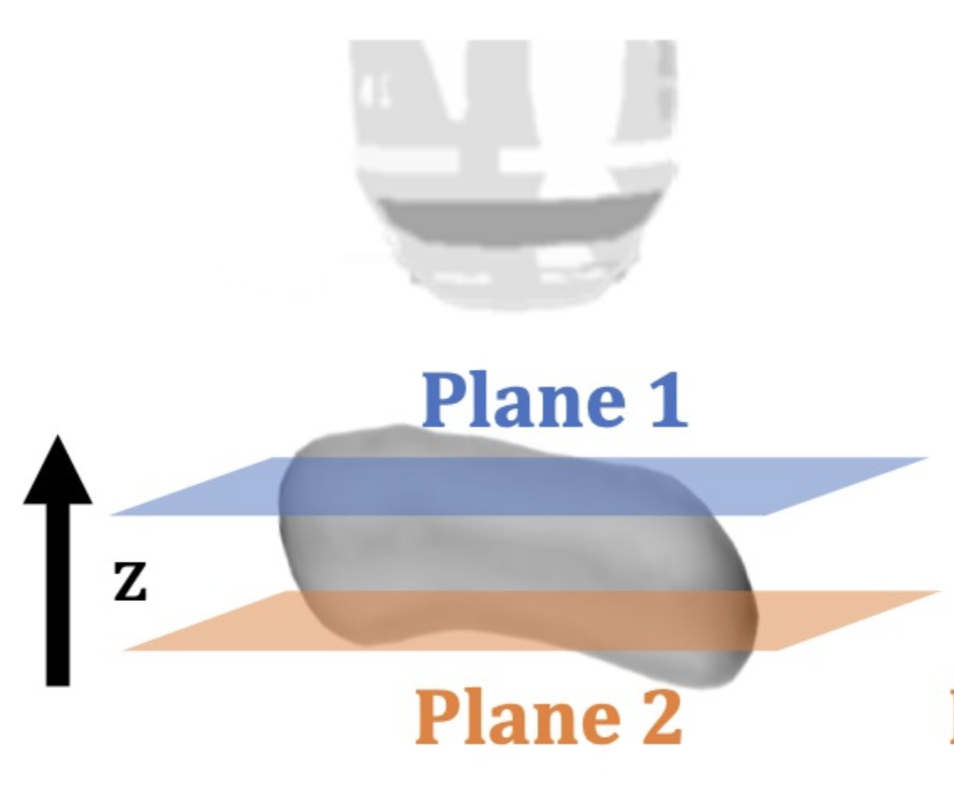
\includegraphics[width=.3\textwidth]{BiPlaneSchematic.png}
\end{center}

\begin{enumerate}
    \item To calibrate the $z$ detection scheme, you will use the file
    \path{Biplane_Calibration_80x80x100nm.tif}.% chktex 29
    This is a multipage TIFF of a
    field of small fluorescent spheres adhered to a glass surface. Between each
    successive page (or slice) of the file, the sample is moved along the $z$
    direction by 59~nm\footnote{Actually, the sample was moved by 100-nm but you
    need to take into account Snell's Law at the glass-water interface between
    the substrate coverglass and the liquid sample. When you do this, you find
    that moving the interface by a distance $\Delta z$ only changes the distance
    between the focus and surface by $0.59 \times \Delta z$. This phenomena,
    called the \textit{Focal Shift}, becomes important for large NA values
    (\url{https://journals.plos.org/plosone/article?id=10.1371/journal.pone.0134616}).}.
    The magnification is such that in the lateral $x,y$ direction, the
    pixels are 80-nm on a side. Open up the file and scan through the slices using Fiji or another viewer of your choice.
    The two planes are both imaged onto the same camera, with the top half of
    the image in a different focal plane than the bottom half. You should see
    that the spatial pattern of bead locations on the top and bottom are the
    same, but that they come into focus at different $z$ positions.

    \begin{center}
        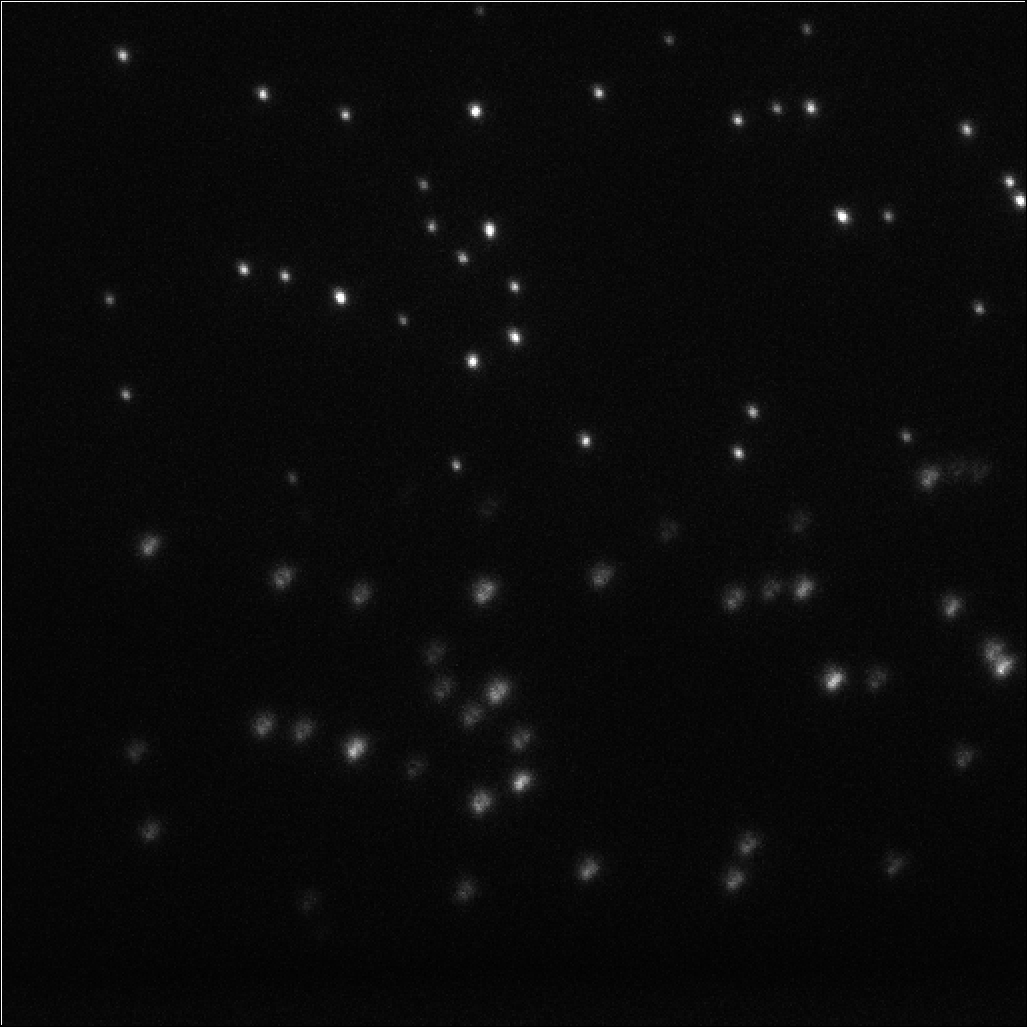
\includegraphics[width=.5\textwidth]{BeadImages.png}
    \end{center}

    Your first step is to identify which beads on the top and bottom correspond
    to each other, i.e.\ you need to \textit{register} the two images by finding a
    mapping from one to the other. An affine transformation is a good start, but
    feel free to explore non-affine affects.

    \item Using this registration mapping, write a program that takes the
    brightness of the center pixel or pixels from the different beads in the two
    halves of the image. For each bead you should have a brightness in the top
    and the bottom as a function of the sample height, $I_{top}(z)$ and
    $I_{bottom}(z)$. Come up with a way of combining these two numbers so that
    you can estimate $z$ from a single top/bottom image pair, i.e.\ find a
    function $f$ such that $z \approx f(I_{top},I_{bottom})$. Also, estimate how
    far apart the two imaging planes are in $z$.

    \item Now open up the file
    \path{Biplane_EcoliGEM_80x80nmx30ms.tif} (warning, this is a large 500MB file).% chktex 29
    This multipage TIFF also has a series of images but for these the sample is
    held fixed and the different slices represent different times taken at a rate
    of one frame per 30~ms, i.e.\ this is a movie. The sample for this movie is a
    field of live \textit{E.~coli} cells that express zero or one
    genetically-encoded nanoparticle. You will also see that there is some weak
    fluorescence from the rest of the cell so that the particles look like bright
    dots on a diffuse background.

    \begin{center}
        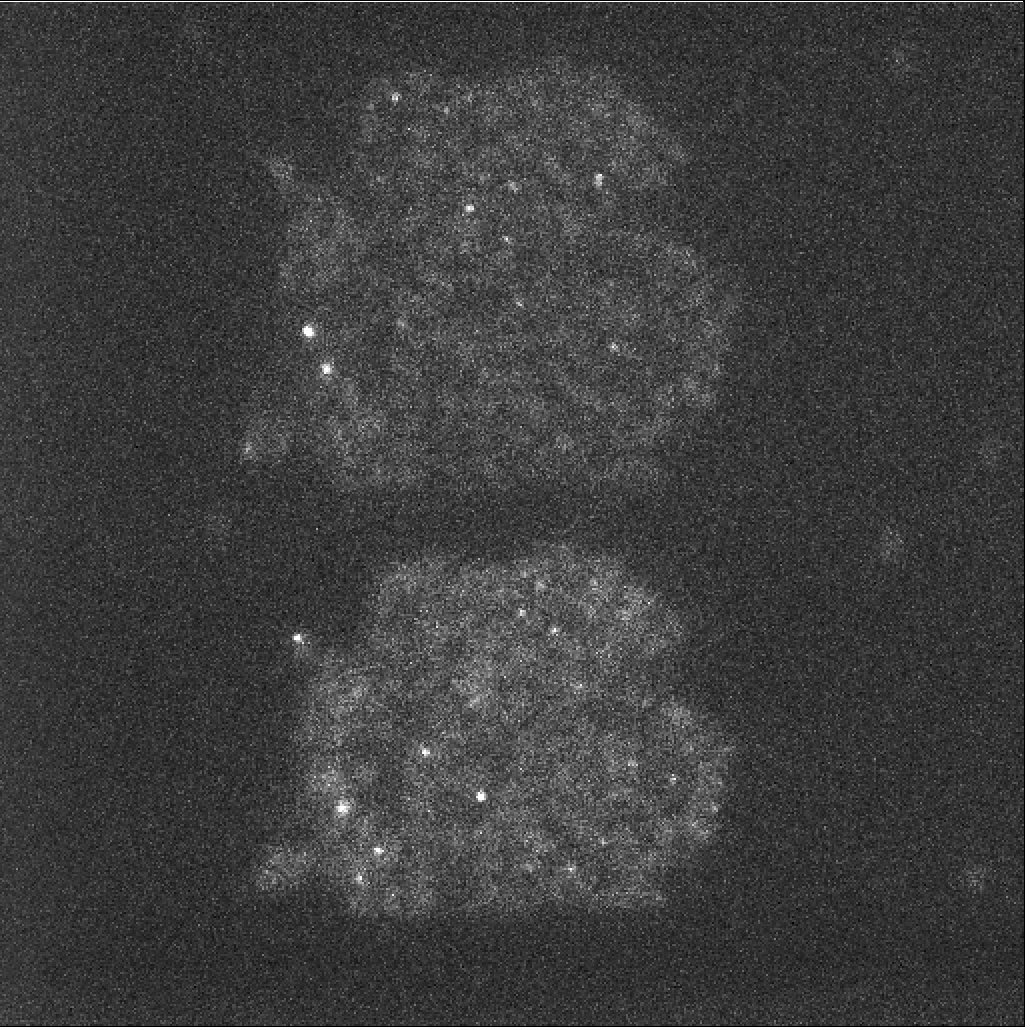
\includegraphics[width=.5\textwidth]{GEMImages.png}
    \end{center}

    Your job is to track the particles in 3D. For this you will need to come up
    with a way to track them in 2D $(x,y)$ and then combine the top/bottom image
    pairs to estimate the $z$ position using your calibration from Part (a). Make graphics that demonstrate the quality of your tracking and report the number of particles you were able to track and the length of the tracks.

\end{enumerate}

\begin{thebibliography}{1}

\bibitem{valverdeMendez2025}
Diana Valverde-Mendez, Alp M.\ Sunol, Benjamin P.\ Bratton, Morgan Delarue,
Jennifer L.\ Hofmann, Joseph P.\ Sheehan, Zemer Gitai, Liam J.\ Holt, Joshua
W.\ Shaevitz, and Roseanna N.\ Zia.
\newblock{} Macromolecular interactions and geometrical confinement determine the
3D diffusion of ribosome-sized particles in live \textit{Escherichia coli}
cells.
\newblock{} \textit{Proceedings of the National Academy of Sciences of the United
States of America}, 122(4):e2406340121, 2025.
\newblock{} \url{https://doi.org/10.1073/pnas.2406340121}.

\end{thebibliography}



\end{document}
